\documentclass[a4paper,11pt]{scrartcl}

\usepackage[ngerman]{babel} 
\usepackage[T1]{fontenc}
\usepackage[utf8]{inputenc}
\usepackage{hyperref}

\usepackage{amsmath,amsfonts,amssymb}
\usepackage{graphicx}
\usepackage{siunitx}

\usepackage{epstopdf}

\setcounter{section}{8}


\begin{document}
\hfill Alexander Schnapp

\hfill Max Menges

\hfill introhpc02

\begin{center}
\underline{\Huge{Intro HPC: Blatt 10}}\\
\large{20.1.2015}\\
\end{center}



\subsection{Matrix multiply-cuda version}
In this exercise a CUDA based implemation of the matrix multiply workload is diskussed. Varying the problem size on the x-axis from 128 to 4096. 
We are calculating with a fixed number of 1024 threads per block. The number of blocks is then calculated out of the problem size.
We compare the CPU computing time with the GPU computing time on the y-axis. Both axes are in logarithmic scale. One can clearly see that the GPU computing time is neglegeble expescially at high problem sizes. The limiting factor by calculation with the gpu is the time to send the data to the gpu and back.

\begin{figure}[htbp]
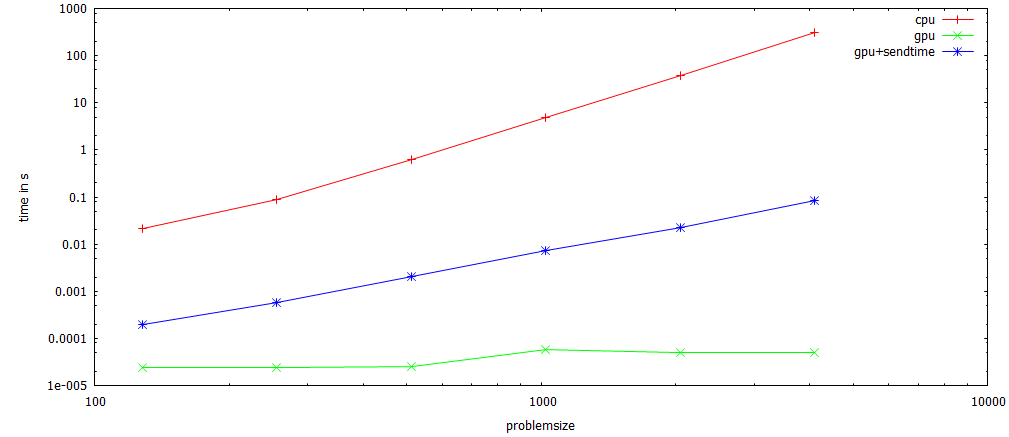
\includegraphics[width=\linewidth,
keepaspectratio]{10.1.test/vergleich}
\centering
\end{figure}

A version which uses shared memory in order to get a even higher speed up is implemented in the code, but does not work yet
\end{document}
